\chapter{Titolo del secondo capitolo}
\label{chap:cap2}

Le assunzioni secondo cui ogni individuo possa entrare in contatto con chiunque (mixing omogeneo) e il numero di interazioni di ciascun soggetto sia confrontabile con quello degli altri non sono realistiche: anzi, la probabilità che si verifichi un incontro fra due individui presi a caso è praticamente infinitesima. Di norma, ognuno ha una serie di contatti regolari con un numero ristretto di persone (familiari, colleghi, etc), mentre ignora tutto il resto della popolazione; questo li rende particolarmente adatti ad essere rappresentati tramite una rete.
\medskip 
Andiamo ad introdurre una serie di definizioni che in seguito ci risulteranno utili. \\
\begin{definizione}[\textit{Grafo}]
Un \emph{grafo} (o una \emph{rete}) è un insieme di elementi detti vertici o \emph{nodi} che possono essere collegati fra loro da segmenti detti archi o \emph{link}.
\end{definizione}
\begin{figure}
		\begin{center}
			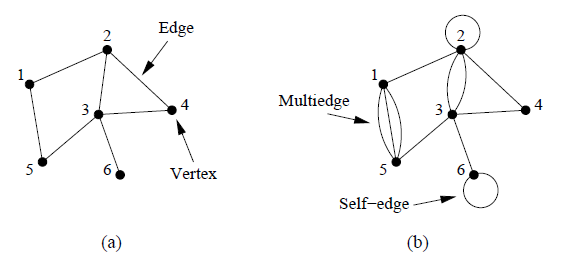
\includegraphics[scale=.8, keepaspectratio]{network_example}
			\caption{(a) Un grafo semplice, cioè privo di loop o link multipli. (b) Un grafo che presenta entrambi. \cite{Newman}}
			\label{fig:net_ex}
		\end{center}
	\end{figure}
	
Consideriamo una rete non orientata - cioè una rete in cui i link possono essere percorsi indistintamente in un verso e nell'altro - con $ n $ vertici, che andiamo ad etichettare da $ 1 $ ... a $ n $. Se indichiamo con $ \left( i, j \right) $ l'arco fra i nodi $ i $ e $ j $, allora l'intera rete può essere descritta in funzione della
\begin{definizione}[\textit{Matrice di adiacenza 1}]
La matrice di adiacenza \textbf{A} relativa ad un grafo semplice è una matrice i cui elementi sono così definiti:
\[
A_{ij} \, =
\begin{cases}
1, & \text{se esiste un arco fra $ i $ e $ j $}\\ 
0, & \text{altrimenti}
\end{cases}
\]
\end{definizione}
Se dunque prendiamo, ad esempio, la rete (a) in \cref{fig:net_ex}, assumerà la seguente forma:
\begin{equation}
A =
\begin{pmatrix}
0 & 1 & 0 & 0 & 1 & 0 \\
1 & 0 & 1 & 1 & 0 & 0 \\
0 & 1 & 0 & 1 & 1 & 1 \\
0 & 1 & 1 & 0 & 0 & 0 \\
1 & 0 & 1 & 0 & 0 & 0 \\
0 & 0 & 1 & 0 & 0 & 0
\end{pmatrix}
\end{equation}
Possiamo osservare che risulta essere una matrice simmetrica con tutti $ 0 $ sulla diagonale. 
\\Qualora invece ne avessimo sotto esame una più simile alla (b) della medesima figura, dovremmo tener conto del fatto che sono presenti link multipli e loop; si stabilisce di assegnare ai primi un numero pari alla loro molteplicità e ai secondi il valore $ 2 $, così che
\begin{equation}
A =
\begin{pmatrix}
0 & 1 & 0 & 0 & 3 & 0 \\
1 & 2 & 2 & 1 & 0 & 0 \\
0 & 2 & 0 & 1 & 1 & 1 \\
0 & 1 & 1 & 0 & 0 & 0 \\
3 & 0 & 1 & 0 & 0 & 0 \\
0 & 0 & 1 & 0 & 0 & 2
\end{pmatrix}
\end{equation}
matrice che rimane, ad ogni modo, simmetrica.
\\La questione cambia leggermente se si va a considerare una rete diretta o \emph{digrafo}.
\begin{definizione}[\textit{Digrafo}]
Un \emph{digrafo} è un tipo di grafo in cui ogni arco ha una direzione, punta cioè da un vertice ad un altro.
\end{definizione}
Ciò ci porta a rivedere quanto detto per la matrice di adiacenza: affermiamo, quindi, che
\begin{definizione}
La matrice di adiacenza \textbf{A} relativa ad un grafo orientato è una matrice i cui elementi sono così definiti:
\[
A_{ij} \, =
\begin{cases}
1, & \text{se esiste un arco da $ j $ a $ i $}\\ 
0, & \text{altrimenti}
\end{cases}
\]
\end{definizione}

\begin{wrapfigure}{l}{0.4\textwidth}
		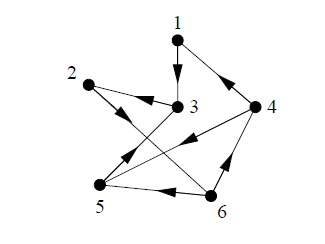
\includegraphics[width=0.38\textwidth]{digraph_example}
		\caption{Un digrafo.}
		\label{fig:dig_ex}
	\end{wrapfigure}
\medskip	
Relativamente alla figura qui a fianco, si avrà
\begin{equation}
A =
\begin{pmatrix}
0 & 0 & 0 & 1 & 0 & 0 \\
0 & 0 & 1 & 0 & 0 & 0 \\
1 & 0 & 0 & 0 & 1 & 0 \\
0 & 0 & 0 & 0 & 0 & 1 \\
0 & 0 & 0 & 1 & 0 & 0 \\
0 & 1 & 0 & 0 & 0 & 0
\end{pmatrix}
\end{equation}